\documentclass[tikz]{standalone}
\usepackage{tikz}
\usetikzlibrary{positioning}
\newcommand{\spacingx}{3cm}
\newcommand{\spacingy}{2cm}
\begin{document}
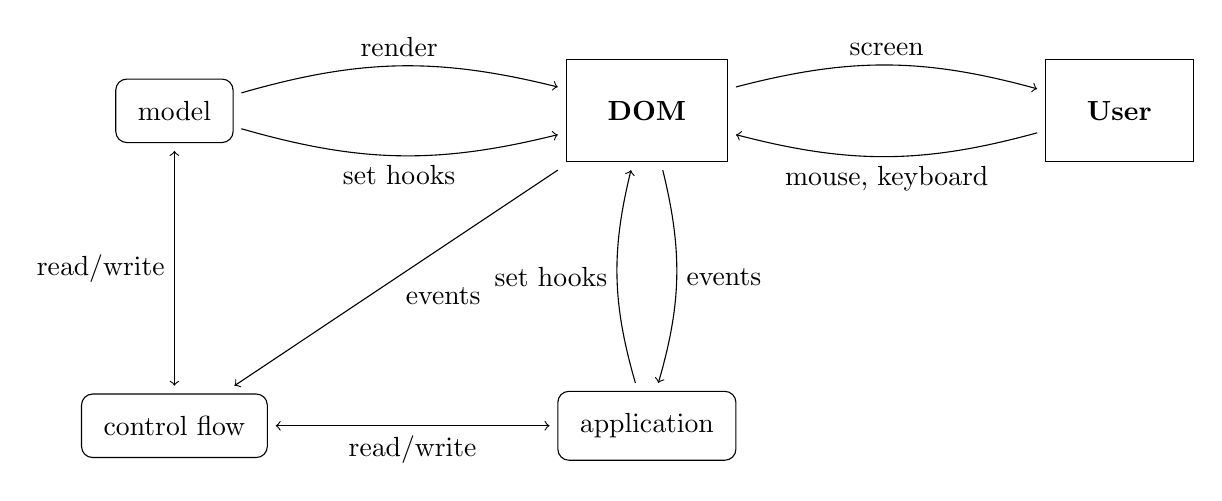
\begin{tikzpicture}[auto]
  \tikzset{state/.style={draw, rounded corners, inner sep=8pt, outer sep=3pt}}
  \tikzset{external/.style={draw, inner sep=15pt, outer sep=3pt}}
  \node[state] (model) at (-\spacingx, \spacingy) {model};
  \node[state] (controlflow) at (-\spacingx, -\spacingy) {control flow};
  \node[state] (application) at (\spacingx, -\spacingy) {application};
  \node[external] (DOM) at (\spacingx, \spacingy) {\bf DOM};
  \node[external] (user) at (9cm, \spacingy) {\bf User};
  \draw (controlflow) edge[<->] node {read/write} (model);
  \draw (controlflow) edge[<->] node[swap] {read/write} (application);
  \draw (DOM) edge[->] node {events} (controlflow);
  \draw (model) edge[->, bend left=15] node {render} (DOM);
  \draw (model) edge[->, bend right=15] node[swap] {set hooks} (DOM);
  \draw (DOM) edge[->, bend left=15] node {events} (application);
  \draw (application) edge[->, bend left=15] node {set hooks} (DOM);
  \draw (DOM) edge[->, bend left=15] node {screen} (user);
  \draw (user) edge[->, bend left=15] node {mouse, keyboard} (DOM);
\end{tikzpicture}
\end{document}
